\chapter{Estudo de Caso}

Neste capítulo será apresentado o estudo de caso sobre a utilização de práticas de usabilidade e testes automatizados no desenvolvimento do Portal do Software Público, baseado na plataforma Noosfero, onde será definido um guia de como essas práticas podem ser inseridas nesse contexto específico.

\section{Objeto de Estudo: Portal do Software Público Brasileiro - SPB}

O Portal do Software Público Brasileiro consiste em um sistema que permite o compartilhamento de softwares e faz parte da política de software livre no setor público.
O SPB será o objeto de estudo de caso, assim como o processo de colaboração com o SPB, que é realizado no LAPPIS da UnB.

\subsection{Visão Geral do Projeto}

O processo de colaboração com o SPB baseia-se no desenvolvimento empírico e nas metodologias ágeis scrum e XP. O desenvolvimento de testes automatizados é intrínseco ao processo de desenvolvimento. A partir destes pontos mencionados, buscamos evoluir a forma com que o processo de colaboraçao com o SPB lida com problemas de usabilidade.
O processo de desenvolvimento é feito a partir de sprints de duas semanas, em que são realizadas reuniões com as equipes e reuniões de planejamento (Planning Poker) em cada equipe para definir as atividades de cada sprint.

%Explicar a dinâmica de trabalho, a equipe, reuniões
%verificar aonde vai entrar essa seção. Talvex dentro do contexto?

\section{Execução do estudo de caso}

\subsection{Problemas encontrados}

No acompanhamento do projeto podemos identificar inicialmente os seguintes problemas relacionados à usabilidade no desenvolvimento de software:

%descrever problemas

	

\subsection{Guia de usabilidade}
%TODO não sei se aplica nesse item (seria o protocolo)
%Melhorar a escrita

	Seguindo as pesquisas realizadas sobre as técnicas de usabilidade e as metodologias existentes propostas por vários autores sobre a integração de tais técnicas em um contexto de desenvolvimento empírico de software, propomos  para este estudo de caso o seguinte guia que deve ser executado nas sprints de desenvolvimento do Portal do Software Público:
	
\begin{enumerate}


\item Análise de Usuários
	
	No ínicio de qualquer projeto é importante conhecer quem são os usuários que irão utilizar o sistema à ser desenvolvido. Para isso existem algumas técnicas que foram identificadas para conhecer melhor quem são os usuários.
	
	A metodologia XPU propõe a criação de Personas e Roteiros para a análise dos usuários, mas além dessas existem outras importantes que podem ser utilizadas no projeto como a utilização de questionário de perfil dos usuários e a análise estatísticas de dados.
	
	\begin{itemize}
		\item \textbf{Personas:} Para a definição de usuários podemos utilizar a técnica de “Persona” que são personagens fictícios criados com base em dados reais. As Personas atuam como representantes dos usuários reais e representam as necessidades de um grupo maior. 
%
A utilização de Personas permite ter um maior foco no usuário, deixando o projeto centrado no usuário. É utilizado para a identificação de requisitos, criação de cenários e \textit{user stories}. 
		\item \textbf{Roteiros:}		
		
		\item \textbf{Questionários de perfil do usuário} Para identificar o perfil dos usuários do Portal do Software Público é necessário realizar uma pesquisa qualitativa para levantamento das principais características contextuais dos usuários típicos, de modo a compreender quem são, qual o conhecimento e experiência com a internet e como utilizam para realizar seu trabalho acadêmico ou profissional. A realização dessa pesquisa será feita com os usuários do antigo Portal do Software Público.
%
A análise do questionário servirá para entender o perfil dos usuários do Portal do Software Público, através da investigação de seus interesses. 

\item \textbf{Dados Estatísticos} Através dos dados estatísticos com ferramentas de análise estatística (\textit{Google analytcs, Piwiki}, entre outros) é possível identificar algumas informações sobre o perfil dos usuários que acessam ao portal. Nas pesquisas quantitativas não são necessários o contato direto com o usuário. Esses dados estatísticos podem ser coletados de base de dados, redes sociais ou sistemas de análises de sites. No caso do portal do software público não foi levado em consideração as questões estatítiscas do portal por se tratar de um novo portal. %TODO Análisar melhor esse paragráfo.

	\end{itemize}
		% acho que é importante colocar um exemplo aqui ou apenas colocar o que será feito no estudo de caso em resultados.?
			
		
\item Análise do contexto de uso

		As Personas e os Roteiros geram as Histórias de usabilidade.

\item Definição de Requisitos e Metas de usabilidade

	Criação de Benchmarks pelos projetistas de interação e usuários para servir como balizadores para avaliar a qualidade da usabilidade que está sendo entregue ao final de cada iteração.
	Baseado nos atributos de usabilidade são estabelecidos instrumentos de medida para se obter valores quantitativos 	para cada atributo.
	Esses benchmarks são utilizados para planejar a avaliação de usabilidade e para realizar os testes que irão compor cada avaliação. % esse paragrafo deve ir pro capitulo de usabilidade onde fala de benchmarks.
	
		
\item Planejamento de Usabilidade

	Estimar os recursos relativos à usabilidade que serão utilizados ao longo do desenvolvimento. Previsões de tempo e custo no planejamento da release.
	 No planejamento da Release do projeto deve-se pensar também em estimativas de tamanho para as histórias de usabilidade e para o planejamento das avaliações de usabilidade.


\item Avaliação da usabilidade

	Ao longo do ciclo de vida diversas avaliações podem ser realizadas:
	
		
	\begin{itemize}
		\item Avaliação Heurística
		
		Antes de executar um teste de usabilidade é importante primeiro fazer uma avaliação heurística para identificar possíveis problemas que possam ser encontrados pelos usuários. Através das Heurísticas de Usabilidade de Nielsen e das listas de verificação, são verificados os problemas inerentes ao Portal do Software Público.
		
%TODO Ver como sera feito no portal do software público.  %Levantamos algumas tarefas/cenários que devem ser executadas para a realização do teste de usabilidade com o objetivo de medir a satisfação relativa a cada tarefa. As tarefas foram pensadas levando em consideração as necessidades dos usuários do Participa.Br. Tarefas que os usuários-alvo executariam mais frequentemente e tarefas que poderiam apresentar problemas para a compreensão e execução do usuário. 
	
		\item Testes com usuários
		
		Em nosso estudo vamos propor que ao final de cada release seja feito um teste de usabilidade com 5 usuários, como é proposto por Nielsen.
				
	\end{itemize} 
	
	As medidas de usabilidade neste estudo foram obtidas considerando-se três fatores: eficácia, eficiência e satisfação de uso.
%
Adotamos como paradigma de avaliação o teste de usabilidade, que consiste em avaliar o desempenho dos usuários na execução de tarefas cuidadosamente preparadas, dentro do escopo do sistema. Esse desempenho pode ser avaliado nos quesitos: número de erros e tempo de execução da tarefa. %Com essa avaliação será coletado tantos dados subjetivos em um cenário real como dados objetivos. Os dados subjetivos serão coletados através de opiniões dos participantes, comentários em relação ao uso do portal da participação social. 
Os dados obtidos consistem em medidas de tempo e desempenho dos participantes.

Elencamos algumas técnicas para avaliar a usabilidade do portal do Software Público:

\begin{table}[h]
\begin{tabular}{|l| p{10cm} |}
\hline
Técnica & Descrição \\ \hline
Observar Usuários & Um observador irá registrar o tempo 
gasto por cada participante para concluir o estudo de caso, 
avaliar a ferramenta e se necessitou de alguma ajuda    \\ \hline
Perguntar aos usuários & Os questionários ASQ e PSSUQ 
de satisfação dos usuários será utilizado 
para coletar as opiniões dos participantes.\\ \hline
\end{tabular}
\caption{Técnicas de avaliação para os testes com usuários}
\end{table}
	
\item Controle de Usabilidade
	
	Ao final de cada interação a velocidade do projeto é avaliada. Deve-se acompanhar as tarefas relativas à usabilidade comparando o esforço previsto com o realizado.
	
\end{enumerate}
Esse protocolo foi extraído do estudo de várias metodologias criadas para a integração das técnicas de usabilidade no contexto de desenvolvimento ágil de software, são elas XPu e XPlus.
 
 
 %TODO Obs: No TCC 1 tinhamos escrito um protocolo de como seria feito á avaliação de usabilidade, algumas coisas podem ser utilizadas e readaptadas para o nosso contexto atual e inserindo as melhorias encontradas por outros métodos.
 
\section{Execução}

%\subsection{Práticas adotadas pela equipe}

\textbf{Questionário Online}

Inicialmente à equipe de design realizou um planejamento para definir o instrumento de pesquisa dos usuários. Foi definido que o principal objetivo do estudo seria medir a percepção dos usuários quanto a qualidade de uso do portal atual sob uma perspectiva global. Nesse sentido foi proposto uma abordagem de pesquisa de levantamento aplicada e quantitativa. A qualidade de uso foi compreendida a partir dos parâmetros propostos pela ISO 9241-10 a 17, como a qualidade da interface de proporcionar eficácia, eficiência e satisfação no uso do portal (APPOLINÁRIO, 2004). 

Na definição do delineamento da pesquisa foi selecionada a técnica de aplicação de questionário on-line para se produzir os dados de opinião dos participantes. Entende-se que a dimensão atitudinal dos usuários do portal com relação a sua experiência de uso só podem ser obtidos por meio do registro de suas verbalizações (MARTINS E THEOPHILO, 2009). No mesmo sentido, a avaliação proposta não permite uma compreensão direta e completa a cerca da usabilidade do portal em si, compreendendo-se que a efetividade do portal só pode ser analisada 
diretamente por meio do uso de outras técnicas de pesquisa, como as observações globais ou sistemáticas da interação entre os participantes e a sua interface % (MARTINS e THEÓPHILO, 2009; ABRAHÃO et al., 2009).

\textbf{Protótipos}
	A equipe utiliza-se de protótipos para determinar os cenários de uso do software, baseando-se nos requisitos definidos pelos clientes. Abaixo estão os protótipos de cadastro de usuário e cadastro de software:

	\begin{figure}[h!]
    	\centering
    	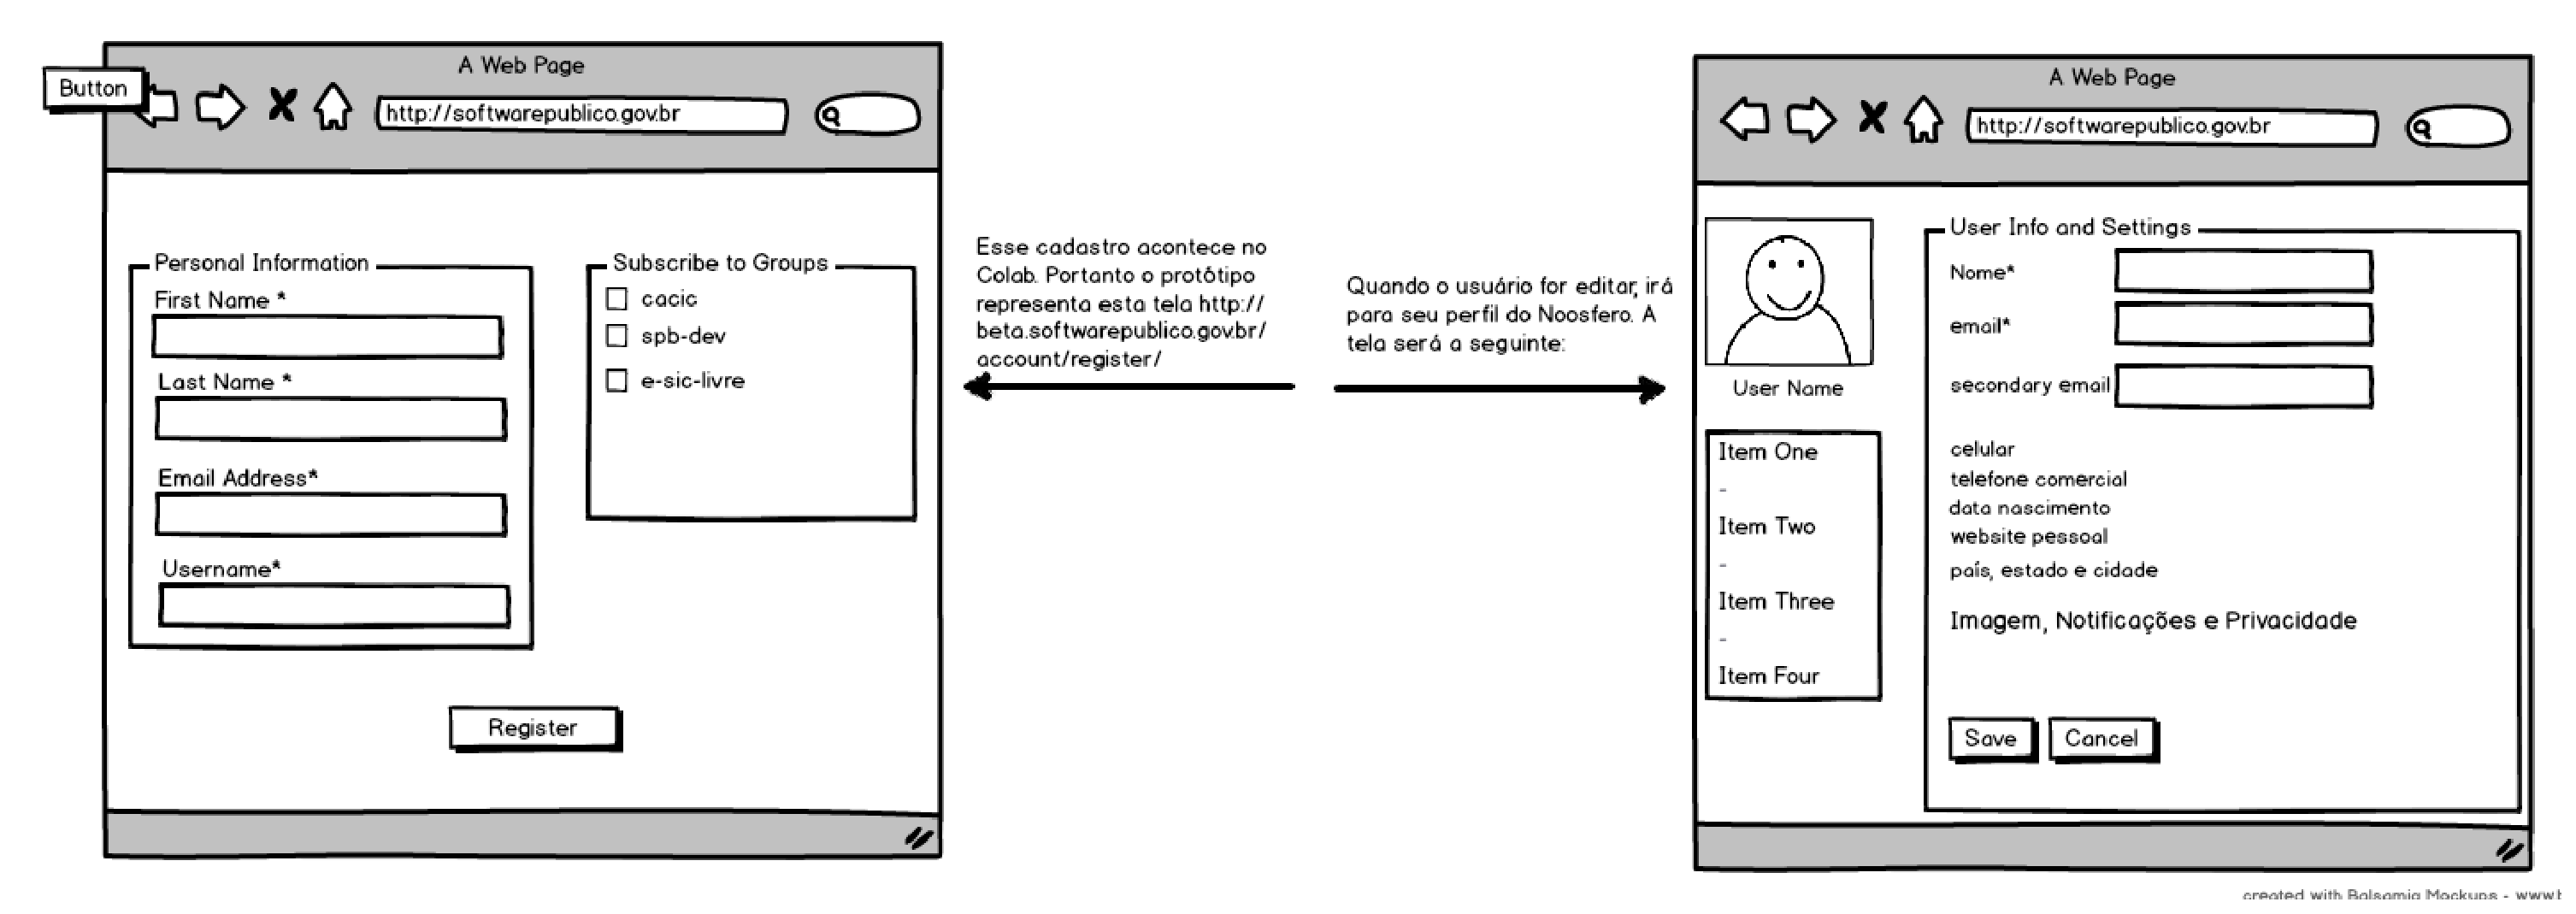
\includegraphics[keepaspectratio=true,scale=0.32]
      		{figuras/CadastroEdicaoUser.eps}
    	\caption{Protótipos de cadastro de usuário}
    	\label{cadastro_user}
	\end{figure}

	\begin{figure}[h!]
    	\centering
    	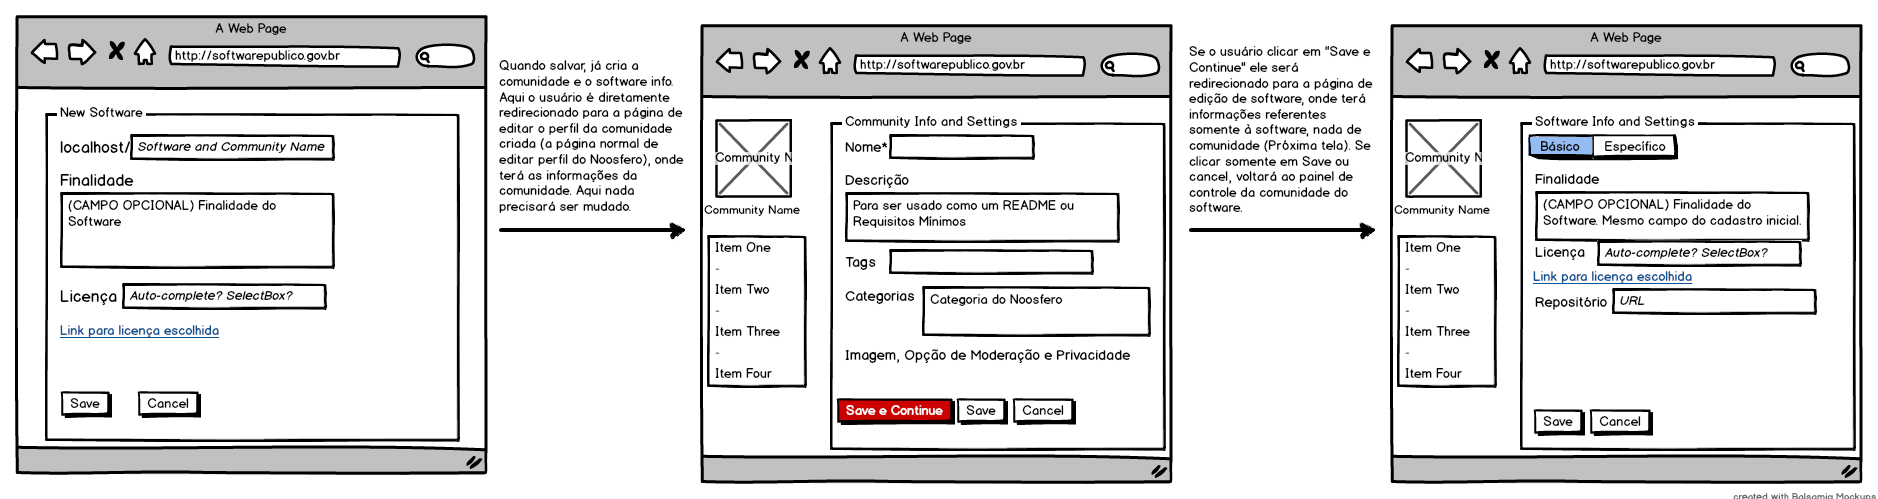
\includegraphics[keepaspectratio=true,scale=0.25]
      		{figuras/CadastroEdicaoSoftware.eps}
    	\caption{Protótipos de cadastro de software}
    	\label{cadastro_software}
	\end{figure}

\newpage

\textbf{Cenários de Uso}
	Para cada funcionalidade desenvolvida é determinado um cenário de uso, base para a implementação dos testes de aceitação e consequentemente o desenvolvimento da funcionalidade propriamente dita.
	Durante a primeira release (release 0) foram desenvolvidas algumas histórias, dentre estas, a história de ``Cadastro de Usuário", que possui os seguintes cenários de sucesso:

	\textbf{Cenário 01:} Cadastro com sucesso de apenas campos obrigatórios
	\textbf{[Dado]} que não existe nenhum usuário com o nome de usuário josesilva 
	\textbf{[Quando]} eu clicar em cadastrar novo usuário
	\textbf{[E]} eu preencho os seguintes campos: 
  		nome de usuário: josesilva
  		e-mail: jose@gmail.com
  		senha: 123456
  		confirmação da senha: 123456
  		nome completo: José da Silva 
  		país: Brasil
  		estado: Distrito Federal
  		cidade: Brasília
	\textbf{[E]} eu clico em cadastrar
	\textbf{[Então]} eu recebo uma confirmação de cadastro realizado com sucesso

	\textbf{Cenário 02:} Cadastro com sucesso de apenas campos obrigatórios de usuário governamental
	\textbf{[Dado]} que não existe nenhum usuário com o nome de usuário josesilva 
	\textbf{[Quando]} eu clicar em cadastrar novo usuário
	\textbf{[E]} eu preencho os seguintes campos: 
  		nome de usuário: josesilva
  		e-mail: jose@serpro.gov.br
  		e-mail secundário: jose@gmail.com
  		senha: 123456
		  confirmação da senha: 123456
		  nome completo: José da Silva 
		  cargo: analista de TI
		  país: Brasil
		  estado: Distrito Federal
		  cidade: Brasília
	\textbf{[E]} eu seleciono ``SERPRO" como instituição
	\textbf{[E]} eu seleciono ``????" como unidade  
	\textbf{[E]} eu clico em cadastrar
	\textbf{[Então]}eu recebo uma confirmação de cadastro realizado com sucesso

\textbf{Cenário 3:} Cadastro com sucesso com todos os campos preenchidos, mesmo não obrigatórios
	\textbf{[Dado]} que não existe um usuário cujo email primário ou email secundário é maria@gmail.com
	\textbf{[Quando]} eu clicar em cadastrar novo usuário
	\textbf{[E]} eu preencho os seguintes campos: 
  		nome de usuário: mariasilva
		  e-mail: maria@gmail.com
		  e-mail secundário: maria@yahoo.com
		  senha: 123456
		  confirmação da senha: 123456
		  nome completo: Maria da Silva
		  cargo: analista de TI
		  áreas de interesse: Engenharia de Software;
		  país: Brasil
		  estado: Distrito Federal
		  cidade: Brasília
	\textbf{[E]} eu seleciono ``Outro" como instituição 
	\textbf{[E]} eu clico em cadastrar
	\textbf{[Então]} eu recebo uma notificação de cadastro realizado com sucesso.

	Os cenários de falha ocorrem nas seguintes situações:
	\begin{itemize}
	\item Email proposto exisitir como email de outro usuário;
	\item Email secundário propostro exisitir como email de outro usuário;
	\item Email secundário ser um email governamental e ao email primário não ser um email governamental;
	\item Não preenchimento de campos obrigatórios para usuário governamental 
	\end{itemize}
%Especificar as datas, as atividades realizadas.


Outra funcionalidade desenvolvida foi a história chamada ``Manter Instituição", que possui os seguintes cenários:

\textbf{Cenário 01:} Cadastro de nova instituição com sucesso
\textbf{[Dado]} que eu estou na página de cadastro de usuário
\textbf{[E]} que a seguinte instituição não existe:
  	nome: Ministério do Planejamento, Orçamento e Gestão
  	sigla: MP
 	poder: executivo
 	esfera: federal
  	tipo: pública
  	cnpj: 00.489.828/0002-36
\textbf{[Quando]} eu clicar em ``Cadastrar nova instituição" 
\textbf{[E]} eu preencher os seguintes campos:
  	sigla: MP
  	poder: executivo
  	esfera: federal
  	tipo: pública
  	cnpj: 00.489.828/0002-36
\textbf{[Então]} eu devo visualizar a mensagem ``Instituição cadastrada com sucesso!"

\textbf{Cenário 02:} Busca de instituição inexistente
\textbf{[Dado]} que eu estou na página de cadastro de usuário
\textbf{[E]} que a seguinte instituição não existe:
  nome: Ministério do Planejamento, Orçamento e Gestão
  sigla: MP
  poder: executivo
  esfera: federal
  tipo: pública
  cnpj: 00.489.828/0002-36
\textbf{[Quando]} eu buscar MP
\textbf{[Então]} eu devo visualizar a mensagem ``Instituição não cadastrada" 
\textbf{[E]}eu devo visualizar a opção de cadastrar nova instituição

Estes cenários apresentam alguns problemas de usabilidade analisando-os de acordo com as heurísticas de Nielsen, e após o processo de desenvolvimento ter uma melhoria na visão de usabilidade após a incorporação de profissionais da área, os cenários apresentaram melhoras em relação às heurísticas de Nielsen. 

Durante a segunda release (release 1) as histórias de ``Cadastro de Usuário", e ``Manter Instituição" foram desenvolvidas novamente com os seguintes cenários:

\textbf{Cenário 01:} Cadastro com sucesso de apenas campos obrigatórios
	\textbf{[Dado]} que não existe nenhum usuário com o nome de usuário josesilva 
	\textbf{[Quando]} eu clicar em ``Cadastre-se"
	\textbf{[E]} eu preencho os seguintes campos: 
  		primeiro nome: José
  		ultimo nome: Silva
  		endereço de e-mail: jose@gmail.com
  		usuário: josesilva
  		
	\textbf{[E]} eu clico em ``Cadastre-se"
	\textbf{[Então]} eu recebo uma confirmação de cadastro realizado com sucesso, com a seguinte mensgamte: 
	``Você deve se logar para seu perfil. Perfis não validados serão deletados em 24h."


Para dar continuidade a este processo este estudo de caso avaliou os cenários estabelecidos e suas evoluções, verificando e propondo melhorias.

Durante a segunda release (release 2) a história de ``Novo Software" foi desenvolvida com os seguintes cenários:

\textbf{Cenário 01:} Novo Software
	\textbf{[Dado]} que não existe nenhum software com o localhost ``software"
	\textbf{[Quando]} eu clicar em ``Novo Software"
	\textbf{[E]} eu preencho os seguintes campos: 
  		localhost: software 
  		finalidade: Finalidade do software
  		licenca: licença
  		
  		
	\textbf{[E]} eu clico em ``Salvar"
	\textbf{[Então]} eu recebo uma confirmação de cadastro realizado com sucesso, e encontro a pagina de edição de software


Outros cenários de edição de software são: ``Informações de Comunidade" e ``Informações de Software".

\textbf{Cenário 02:} Informações de Comunidade
	\textbf{[Dado]} que ``software" está cadastrado
	\textbf{[Quando]} eu clicar em ``Cadastre-se"
	\textbf{[E]} eu preencho os seguintes campos: 
  		descricao: Descricao do software 
  		tags: software
  		categorias: categoria1
 
	\textbf{[E]} eu clico em ``Salvar"
	\textbf{[Então]} eu recebo uma confirmação de cadastro salvo com sucesso


\textbf{Cenário 03:} Informações de Software
	\textbf{[Dado]} que ``software" está cadastrado e estou em Edição de software
	\textbf{[Quando]} eu clicar em ``Especifico"
	\textbf{[E]} eu preencho os seguintes campos: 
  		Sigla: teste 
  		sistema operacional: teste os
  		funcioanalidades: testes
  		categorias: categoria1
 	
 	\textbf{[E]} eu clico em ``Nova Biblioteca"
 	\textbf{[E]} eu preencho os seguintes campos: 

 		nome: teste
 		versao: teste
 		licenca: teste

 	\textbf{[E]} eu clico em ``Novo Sistema Operacional"
 	\textbf{[E]} eu preencho os seguintes campos: 

 		nome: Debian
 		versão: teste
 	\textbf{[E]} eu clico em ``Nova linguagem"
 	\textbf{[E]} eu preencho os seguintes campos: 

 		nome: C++
 		versão: teste
 		sistema operacional: Debian
 	\textbf{[E]} eu clico em ``Novo Banco de Dados"
 	\textbf{[E]} eu preencho os seguintes campos: 

 		nome: apache
 		versão: teste
 		sistema operacional: Debian
	\textbf{[E]} eu clico em ``Salvar"
	\textbf{[Então]} eu recebo uma confirmação de cadastro salvo com sucesso


\section{Análise e Interpretação dos Resultados}

Esta seção apresenta a discussão e a interpretação dos resultados observados durante a execução do estudo de caso descrito.

Analisando os protótipos e os cenários de uso desenvolvidos, de acordo com as heurísitcas de Nielsem, encontramos alguns problemas de usabilidade e propomos melhorias a serem feitas e possivelmente verificadas durante os testes de aceitação.

\subsection{Análise dos Dados}

Baseado nos objetivos do estudo de caso, os dados a serem levantados dizem respeito à ???

\subsection{Análise dos Resultados de Medição}

Analisa os resultados alcançados no estudo de caso, baseado ...

\subsection{Verificação}

Esta subseção analisa os resultados alcançados no estudo de caso, baseado nas hipóteses levantadas e apresentadas no ínicio desta seção........


\section{Considerações finais do capítulo}







